\section{}

I used a burn in of 20 and a thinning stride of 4.
The plot of the samples along with the contour plot can be seen in Figure \ref{fig:gibbs_samples}.
When I calculated the posterior means by hand I got $\expec{X1|X2} = \mu_1 - .75(x_2 - 2)$, but this caused a negative correlation in the variables so I manually flipped the sign.
Still, I'm unsure where my calculation went wrong.

The trace plot for the first variable (mean=0) is in Figure \ref{fig:x1_trace} and the autocorrelation (after thinning) for the same variable is in Figure \ref{fig:x1_autocorr}.



\begin{figure}
     \centering
     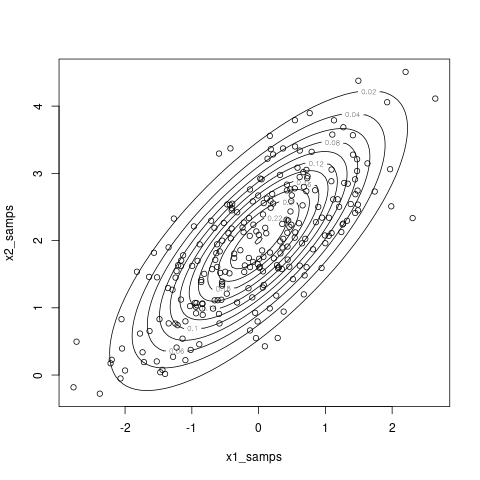
\includegraphics[width=.50\textwidth]{../code/q2/plots/gibbs_samples.png}
     \caption{Results of Gibbs sampling.}
     \label{fig:gibbs_samples}
\end{figure}
\begin{figure}
     \centering
     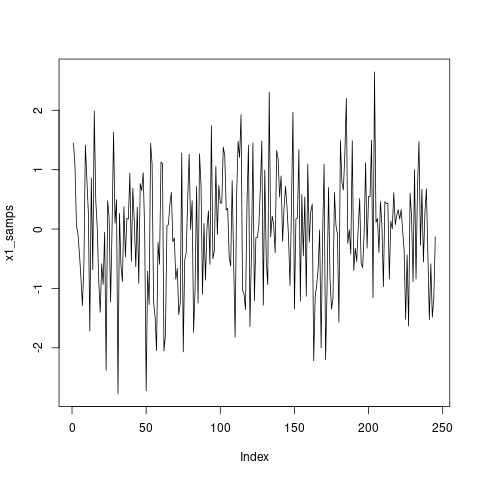
\includegraphics[width=.50\textwidth]{../code/q2/plots/x1_trace_plot.png}
     \caption{Trace plot of the MCMC samples from the first variable}
     \label{fig:x1_trace}
\end{figure}
\begin{figure}
     \centering
     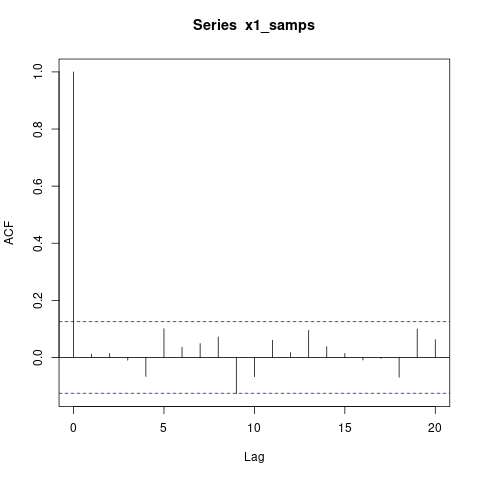
\includegraphics[width=.50\textwidth]{../code/q2/plots/x1_lag1_autocorr.png}
     \caption{Autocorrelation plot of the MCMC samples of the first variable}
     \label{fig:x1_autocorr}
\end{figure}
